
\chapter{Ant Colony Optimization}

The \textit{Ant Colony Optimization (ACO)} algorithm is a probabilistic optimization metaheuristic first presented by Dorigo and Stützle \cite{Dorigo2010}. The algorithm is based on the behavior of ants. When searching for food, multiple ants scatter around their anthill. They lay down small amounts of pheromone to remember the way back. If their search is successful, they return to the anthill while laying down a much stronger layer of pheromone to mark the path to the finding. Other ants can then follow this pheromone trail instead of searching randomly. The pheromone, however, slowly evaporates, so the trail gets thinner for longer paths. This allows the ants to find the shortest paths to nearby food.

The \textit{ACO} builds on this metaphor. Our \textit{ants} generate possible solutions by moving through the \textit{parameter space}. When they create a solution, they update the \textit{pheromone} stored in the \textit{pheromone matrix} based on the fitness value of their solution. When new ants then move through the parameter space, they follow paths with higher pheromone levels, increasing the chance of finding a better solution. Apart from the pheromone levels, the ant also decides on the heuristic value of the path - \textit{attractiveness}.

We represent our \textit{parameter space} as an oriented graph. Vertices are the group's pick-ups and drop-offs. Edges represent the traveling, e.g., the edge between the group’s $i$ drop-off and the group’s $j$ pick-up represents the path between the group’s $i$ destination point and the group’s $j$ departure point. We must also add a node for the depot. The solution is then a set of paths through the graph, where each path satisfies the constraints defined in \ref{constraints}.

\section{Creating solutions}

An \textit{ant} generates new routes until all the customer requests are handled. Each route starts by picking up the first unhandled group with the lowest departure time. We then create a set of all possible options: pick up a new group, drop off a group sitting in the bus, and, only if the bus is empty, return to the depot. The probability of picking each option is based on the amount of pheromone between the two nodes $\tau$ and the attractiveness value of the transition $\nu$. The probability of transition from vertex $i$ to vertex $j$ is then proportional to $\tau_{ij}^\alpha \cdot \nu_{ij}^\beta$, where $\alpha$ and $\beta$ are hyperparameters specifying the ratio between $\tau$ and $\nu$. If the option to return to the depot is selected, the route ends.

\subsubsection{Attractiveness}

We use a simplified heuristic used in section \ref{sec:evoh}. The attractiveness is equal to a weighted sum of the travel time between the stops and the time window violation - how soon or late would the bus arrive.

When considering dropping off a group, we can adjust the attractiveness by multiplying it with a \textit{drop-off attractiveness bonus} hyperparameter. Setting it high can force the ants to drop off groups as soon as possible to minimize delays while setting it low helps fill the bus's capacity, which can sometimes minimize travel times. We define this coefficient as a function taking the current route and the \textit{ant's id}. The \textit{ant's id} parameter can be useful for assigning different strategies to different ants, and passing the route allows one to make decisions based on its length.

When calculating attractiveness for returning to the depot, we have no time window to consider in the weighted sum. Instead, we only multiply the travel time to the depot with the \textit{depot attractiveness coefficient} hyperparameter to favor or disfavor the depot and, therefore, end the current route. This coefficient is also defined as a function taking the current route.

\section{Pheromones}

The pheromone matrix is of size $(2|G| + 1) \times (2|G| + 1)$, where $G$ is the set of all groups. For each group with id $i$, the pheromone at index $i$ represents the probability of the group being picked up, and the pheromone at index $i + |G|$ represents the likelihood of the group being dropped off. The last index represents the depot. We initialize it at the beginning of the algorithm uniformly.

After all the ants generate their solutions, we need to update the pheromone matrix. Firstly, we \textit{evaporate} the current pheromone by setting the matrix to $\tau = (1 - \rho)\tau$, where $\rho$ is a hyperparameter. Then, we update the pheromones based on the generated solutions and their fitness values. The update is defined as $\Delta\tau_{ij} = \sum_{k=1}^{ants}\Delta\tau_{ij}^{k}$, where
\begin{equation}
    \Delta\tau_{ij}^{k} = 
        \begin{cases}
        Q / L_k & \text{if edge $ij$ was used in the $k$th solution} \\
        0 & \text{otherwise}
        \end{cases}
\end{equation},
$Q$ is a hyperparameter and $L_k$ is the fitness value of the $k$th solution.

After updating the pheromone matrix, we start a new iteration by generating new solutions for each ant. This is done until the iteration limit is reached or until the algorithm stops converging (all ants are generating the exact same solution for many iterations).

\section{Hyperparameters}\label{sec:aco_hyperparams}

The hyper-parameter settings for both dataset types were chosen experimentally and are shown in the table \ref{tab:aco_hyperparams}. 

The experiments were done the same way as in the section \ref{sec:genetic_hyperparams}. For example, in figure \ref{fig:aco_alpha_beta}, we show experiments for setting the $\alpha$ and $\beta$ parameters. We can see that using higher $\alpha = 2$ (or higher) leads to converging to non-optimal solutions. On the \textit{random} dataset, after about 1000 iterations, the algorithm converged to a local optimum and the generated solutions were all the same, so the runs terminated prematurely.

For the random dataset, we set the \textit{drop-off attractiveness bonus} as $50.0$ to motivate dropping the customers off as soon as possible to reduce their delays. For the commute dataset, we set it based on the route's current length - if the route is shorter than a random number between 3 and 5, we set it as $0.1$ to prefer picking up another group. If it is longer, we set it as $100.0$. As a result, the solution contains routes where each bus picks between 3 to 5 groups in the first area and then drops them all off in the destination area. Values 3 and 5 were chosen experimentally, and they depend mostly on the distance between the departure and destination areas and the density of requests in time.

We do not use the \textit{ant\_id} parameter in \textit{drop-off attractiveness bonus} for the final experiments since we failed to find a combination of strategies that would work better than the single strategy used. For example, combining the strategy used for the random dataset with the current one results in finding a local optimum, where the number of buses is close to the number of requests and each bus handles only at most 2 requests.

For the commute dataset, the value of the \textit{depot attractiveness coefficient} does not have much impact on the results - after dropping off all the groups in the destination area, the attractiveness of picking up any group in the source area is too low because the group would be picked up too late, while the depot attractiveness stays high. However, for the random dataset, a lower value, such as $0.1$, lowers the number of buses used. This can be because we only consider returning to the depot when the bus is empty, but we do not penalize the waiting of an empty bus. The attractiveness function, however, still considers the time window violation, so if the bus were to wait for a long time, it would rather return to the depot. While we still need to account for the time windows since picking up groups with earlier departure times might be more favorable, we do not want their attractiveness to be significantly lower than the depot's attractiveness, which does not have a time window. Therefore, lowering the depot attractiveness by multiplying it with a small fixed constant works well.

\begin{figure}
    \centering
    \begin{subfigure}[b]{0.45\textwidth}
        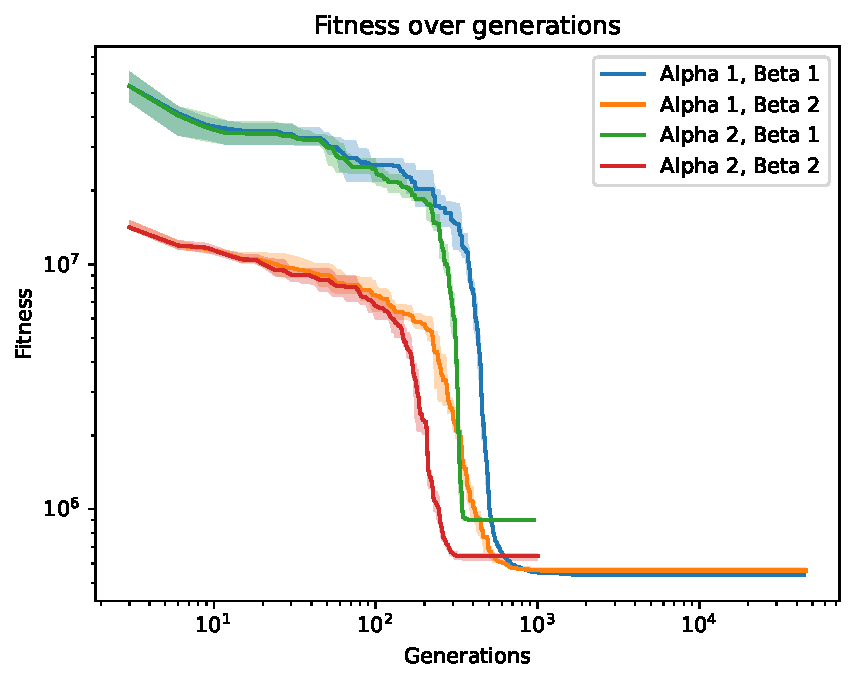
\includegraphics[width=\textwidth]{img/aco_random_ab.pdf}
        \caption{Randomly distributed data}
        \label{fig:aco_ab_random}
    \end{subfigure}
    \begin{subfigure}[b]{0.45\textwidth}
        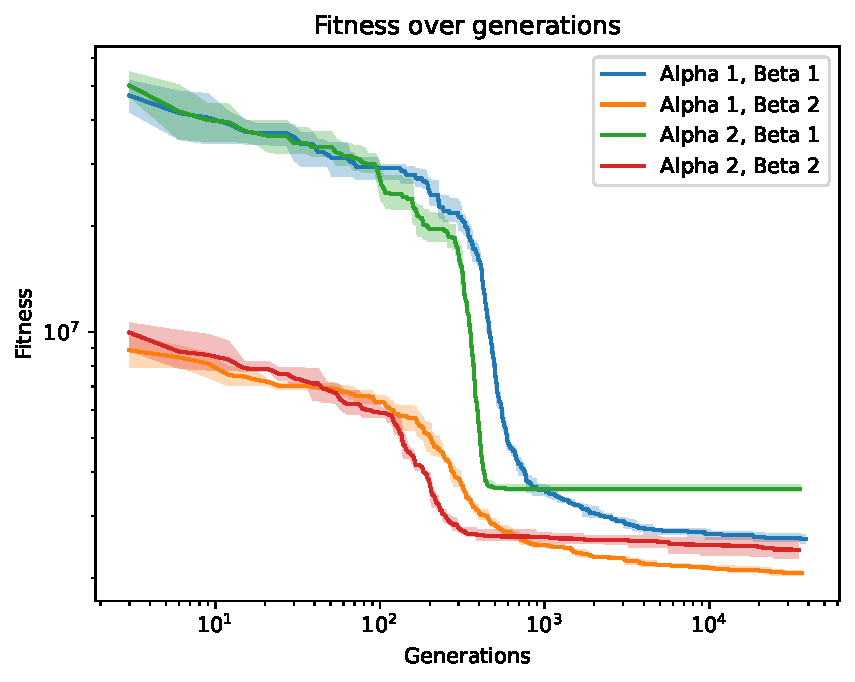
\includegraphics[width=\textwidth]{img/aco_commute_ab.pdf}
        \caption{Long distance commute data}
        \label{fig:aco_ab_commute}
    \end{subfigure}
    \caption{Ant Colony Optimization - Alpha and Beta setting}
    \label{fig:aco_alpha_beta}
\end{figure}

\begin{table}
    \centering
    \begin{tabular}{lcc}
         & Random & Commute \\
        \hline
        $\alpha$ & \multicolumn{2}{c}{1} \\
        $\beta$ & 1 & 2 \\
        $\rho$ & \multicolumn{2}{c}{0.01} \\
        $Q$ & \multicolumn{2}{c}{10 000} \\
        Travel time weight in heuristic cost & 1 & 2 \\
        Time window violation weight in heuristic cost & 2 & 1 \\
        Time window size & 0.01 & 0.1 \\
        Depot attractiveness coefficient & \multicolumn{2}{c}{0.1}
    \end{tabular}
    \caption{Ant Colony Optimization - hyper-parameter settings}
    \label{tab:aco_hyperparams}
\end{table}